\documentclass[dvipdfmx]{jarticle}
\pagestyle{empty}
\usepackage{fancyvrb}
\usepackage{tikz}
\usetikzlibrary{shapes,calc,arrows.meta}
\begin{document}
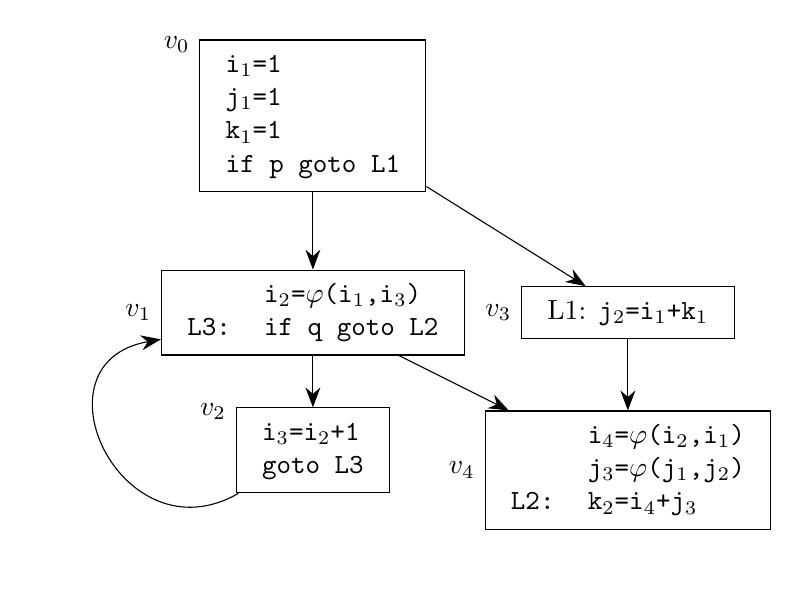
\begin{tikzpicture}
    \node[draw,rectangle,label={155:{$v_0$}}] (v0) at (0,0) {\begin{tabular}{l}
            \verb|i|$_1$\verb|=1| \\
            \verb|j|$_1$\verb|=1| \\
            \verb|k|$_1$\verb|=1| \\
            \verb|if p goto L1|
        \end{tabular}};
    \node[draw,rectangle,label={180:{$v_1$}}] (v1) at (0,-2.5) {\begin{tabular}{ll}
                       & \verb|i|$_2$\verb|=|$\varphi$\verb|(i|$_1$\verb|,i|$_3$\verb|)| \\
            \verb|L3:| & \verb|if q goto L2|
        \end{tabular}};
    \node[draw,rectangle,label={165:{$v_2$}}] (v2) at (0,-4.25) {\begin{tabular}{l}
            \verb|i|$_3$\verb|=i|$_2$\verb|+1| \\
            \verb|goto L3|
        \end{tabular}};
    \node[draw,rectangle,label={180:{$v_3$}}] (v3) at (4,-2.5) {\begin{tabular}{l}
            L1: \verb|j|$_2$\verb|=i|$_1$\verb|+k|$_1$
        \end{tabular}};
    \node[draw,rectangle,label={180:{$v_4$}}] (v4) at (4,-4.5) {\begin{tabular}{ll}
                       & \verb|i|$_4$\verb|=|$\varphi$\verb|(i|$_2$\verb|,i|$_1$\verb|)| \\
                       & \verb|j|$_3$\verb|=|$\varphi$\verb|(j|$_1$\verb|,j|$_2$\verb|)| \\
            \verb|L2:| & \verb|k|$_2$\verb|=i|$_4$\verb|+j|$_3$
        \end{tabular}};
    \path[-{Stealth[scale=1.5]}] (v0) edge (v1) (v0) edge (v3);
    \path[-{Stealth[scale=1.5]}] (v1) edge (v2) (v1) edge (v4);
    \path[-{Stealth[scale=1.5]}] (v3) edge (v4);
    \path[-{Stealth[scale=1.5]}] (v2) [out=210,in=190,looseness=2.0] edge (v1);
\end{tikzpicture}
\end{document}